\documentclass[twoside]{report}
\usepackage{iwsm}
\usepackage{graphicx}
\usepackage{amsmath, amssymb, bm}
\usepackage{booktabs}
\usepackage{lipsum}  
% Please do not specify any new definitions, any new commands,
% and do not specify any style parameters.
% The preamble of the document should be left unchanged.

\begin{document}

%***********************************************************************
% PLEASE INSERT YOUR CONTENT FROM HERE
%***********************************************************************

% Title and running title to be used as left header:
\title{Forecasting vital rates from demographic summary measures}
\titlerunning{Forecasting vital rates}

% Authors and running list of authors to be used as right header:
\author{Carlo G.~Camarda\inst{1}}
\authorrunning{Camarda}    %% use \authorrunning{Surname 1} if only 1 author
                                    %% use \authorrunning{Surname 1 and Surname2} if two authors
                                    %% use \authorrunning{Surname 1 et al.} if more than two authors

% Institutes of all authors
% Include city and country of each institute, do not include the full address.
\institute{Institut national d'\'{e}tudes d\'emographiques (INED), Paris, France}

% E-mail of presenting author for correspondence
\email{carlo-giovanni.camarda@ined.fr}

% Brief abstract of the paper:
\abstract{In population and actuarial sciences, time-trends of summary measures (such as life expectancy or the average number of children per woman) are easy to interpret and predict. Most summary measures are nonlinear functions of the vital rates, the key variable we usually want to estimate. Furthermore smooth outcomes of future age-specific vital rates are desirable. Therefore, optimization with nonlinear constraints in a smoothing setting is necessary. We propose a methodology that combines Sequential Quadratic Programming and a $P$-spline approach, allowing to forecast age-specific vital rates when future values of demographic summary measures are provided.
We provide an application of the model on Japanese mortality and Spanish fertility data.}

% Keywords (at most 5):
\keywords{Vital rates forecast; Smoothing; Constrained nonlinear optimization; Summary measures.}

% Produce the title:
\maketitle

%***********************************************************************

% Sections and subsections (do not use lower levels):

\section{Introduction}
Future mortality and fertility levels can be predicted by either modelling and extrapolating rates over age and time, or by forecasting summary measures, later converted into age-specific rates. 
The latter approach takes advantage of the prior knowledge that demographers and actuaries have on possible future values of life expectancy at birth and total fertility rates. For instance, this methodology has been lately adopted by the United Nations (\v{S}ev\v{c}\'ikov\'a et al., 2016). 
In this paper, we propose a model to obtain future mortality and fertility age-patterns which comply with the projected summary measures. Unlike comparable approaches, we assume only smoothness of future vital rates which is achieved by a two-dimensional $P$-spline approach as in Currie et al.~(2004). Since summary measures are commonly nonlinear functions of the estimated penalized coefficients, Lagrangian multipliers cannot be directly implemented. We hence opted for a Sequential Quadratic Programming (SQP) procedure (Nocedal \& and Wright, 2006) to perform the associated constrained nonlinear optimization.
We illustrate our approach with two data sets: mortality of Japanese females, based on future life expectancy predicted by UN World Population Prospects (2017) and Spanish fertility constrained to total fertility rates, mean and variance of age at childbearing derived by classic time-series analysis.

\section{Model on Japanese mortality data}

For ease of presentation, we formulate the model on mortality data. We suppose that we have deaths, and exposures to risk, arranged in two matrices, 
$\bm{Y} = (y_{ij})$ and $\bm{E} = (e_{ij})$, each $m \times n_{1}$, whose rows and columns are classified by age at death, $\bm{a}, \,m \times 1$, and year of death, $\bm{t}_{1}, \,n_{1} \times 1$, respectively.  
We assume that the number of deaths $y_{ij}$ at age $i$ in year $j$ is Poisson distributed with mean $\mu_{ij} \,e_{ij}$. %The value of $\mu_{ij}$ is commonly named force of mortality. 
Forecasting aims to reconstruct trends in $\mu_{ij}$ for $n_{2}$ future years, $\bm{y}_{2}, n_{2} \times 1$.

Usually demographers and actuaries summarize mortality age-patterns by computing life expectancies. Time-trends of this summary measure are often regular and well-understood. Forecasting a single time-series is therefore relatively easy. Figure~\ref{fig:CamardaMort} (left panel) presents observed life expectancy at age 1 for Japanese females from 1960 to 2016 along with the medium variant up to 2050 as computed by the UN, which consider available data for all countries in the world.  
Future mortality patterns, both by age and over time, must adhere to this predicted trend. 

\begin{figure}[!ht]\centering
	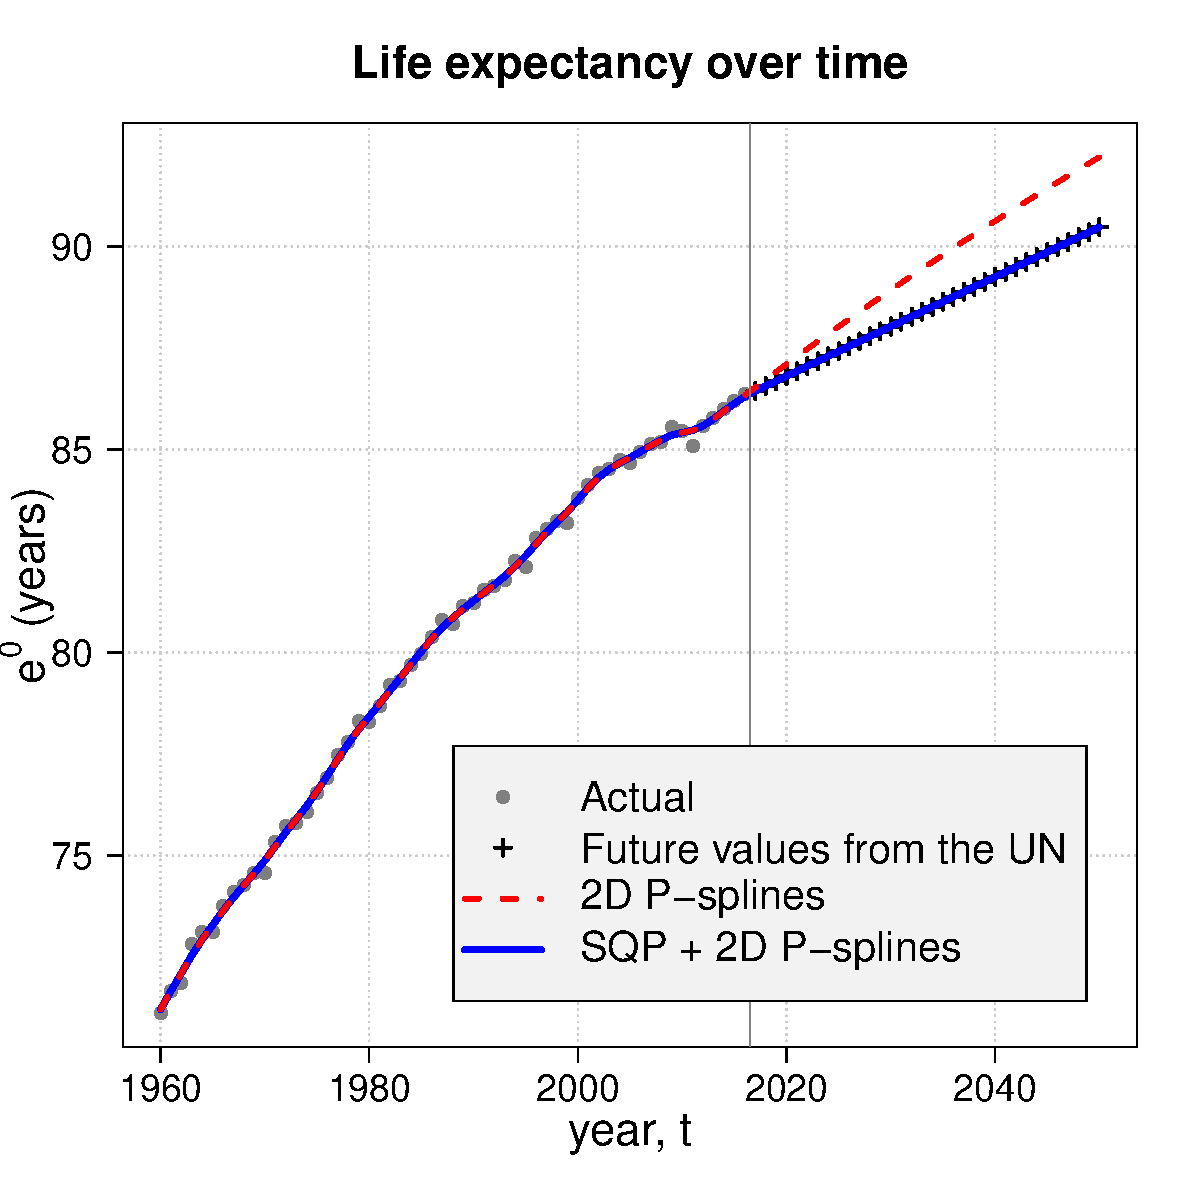
\includegraphics[scale=0.25]{CamardaE0.pdf}
	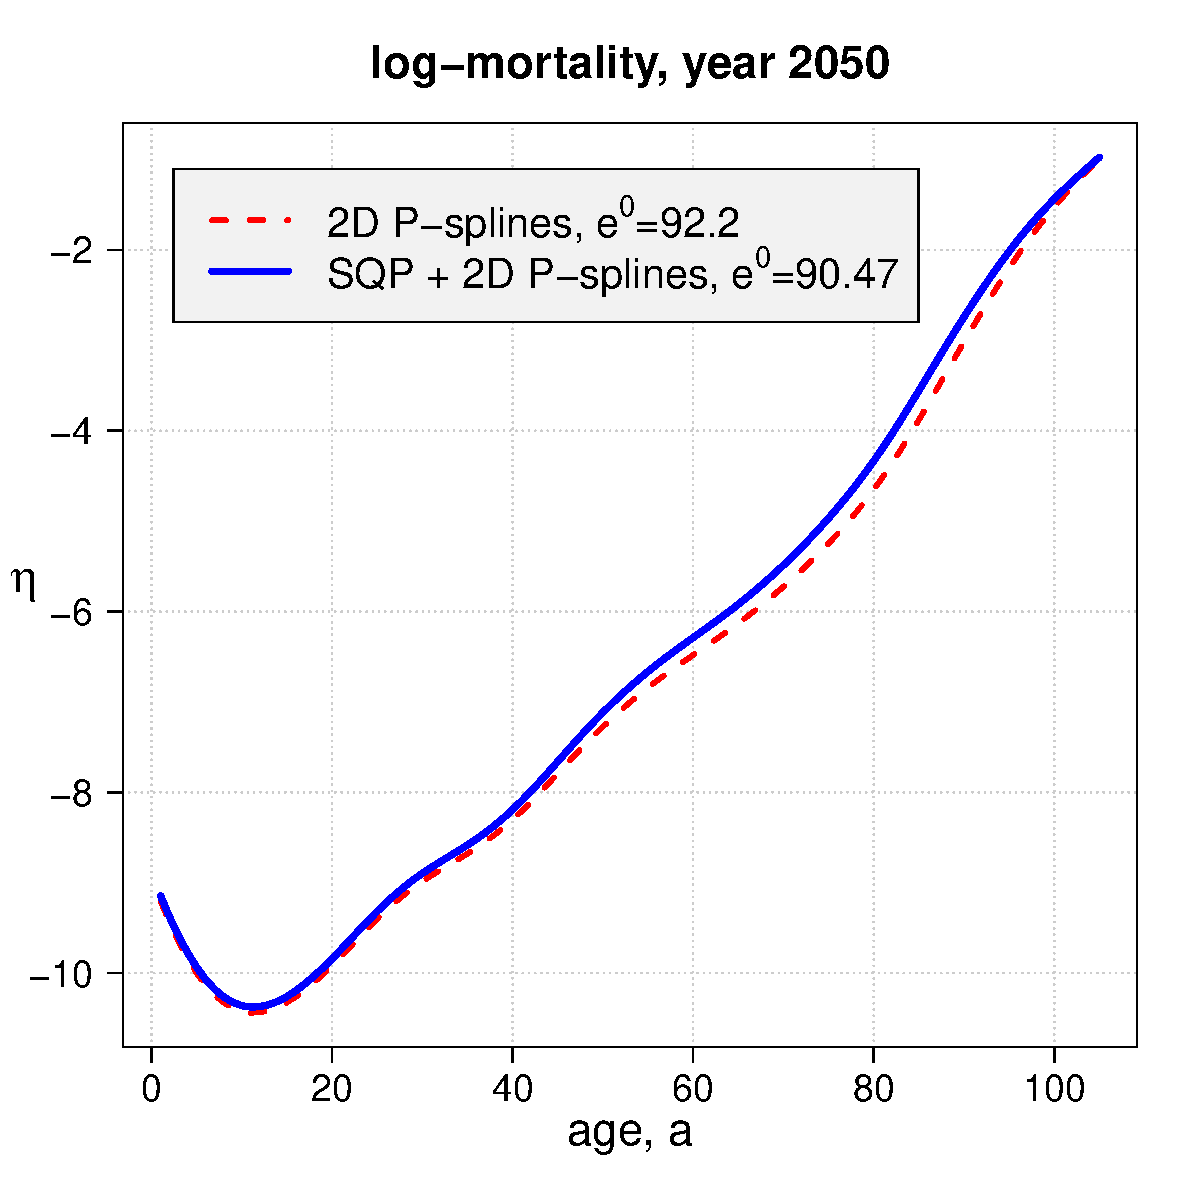
\includegraphics[scale=0.25]{CamardaMort2050.pdf}
	\caption{\label{fig:CamardaMort} Left panel: Actual, estimated and forecast life expectancy at age 1 by United Nations, 2D $P$-splines and the SQP+2D $P$-splines. Right panel: Mortality age-pattern in 2050 by 2D $P$-splines and the SQP+2D $P$-splines. Japanese females, ages 1-105, years 1960-2016, forecast up to 2050.}
\end{figure}

We arrange data as a column vector, that is, $\bm{y} = \verb"vec"(\bm{Y})$ and $\bm{e} = \verb"vec"(\bm{E})$ and we model our Poisson death counts as follows: $\bm{\eta} = \ln(E(\bm{y})) = \ln(\bm{e})+ \bm{B}\,\bm{\alpha}\, , $ where $\bm{B}$ is the regression matrix over the two dimensions: $\bm{B} = \bm{I}_{n_{1}} \otimes \bm{B}_{a}$, with $\bm{B}_{a} \in \mathbb{R}^{m \times k_{a}}$. Over time, we employ an identity matrix of dimension $n_{1}$ because we will incorporate a constraint for each year. In order to forecast, data and bases are augmented as follows:
\begin{equation}\label{eq:AugData}
\breve{\bm{E}} = [\bm{E} : \bm{E}_{2}]\, , \qquad 
\breve{\bm{Y}} = [\bm{Y} : \bm{Y}_{2}]\, , \qquad
\breve{\bm{B}} = \bm{I}_{n_{1}+n_{2}} \otimes \bm{B}_{a}
\, ,
\end{equation}
where $\bm{E}_{2}$ and $\bm{Y}_{2}$ are filled with arbitrary future values. If we define a weight matrix $\bm{V} = \mathrm{diag}(\verb"vec"(\bm{1}_{m\times n_{1}}:\bm{0}_{m\times n_{2}}))\,$, the coefficients vector $\bm{\alpha}$
can be estimated by a penalised version of the iteratively reweighted least squares algorithm: 
\begin{equation}\label{eq:penIRWLSfor}
(\breve{\bm{B}}^{T} \bm{V} \tilde{\bm{W}} \breve{\bm{B}} + \bm{P}) \tilde{\bm{\alpha}} =
\breve{\bm{B}}^{T}\bm{V} \tilde{\bm{W}}\tilde{\bm{z}} \, ,
\end{equation} 	
where a difference penalty $\bm{P}$ enforces smoothness behaviour of mortality both over age and time. Outcomes from this approach in terms of life expectancy is depicted with a dashed red line in Figure~\ref{fig:CamardaMort} (left panel), and a departure from the UN projected values is evident. 

Life expectancy is a nonlinear function of the coefficients vector $\bm{\alpha}$:
\begin{equation}\label{eq:e0}
\bm{e}^{0} (\bm{\alpha}) = (\bm{1}_{1 \times m} \otimes \bm{I}_{n}) \, \exp[ (\bm{I}_{n} \otimes \bm{C}) \verb"vec"(\exp(\bm{B}\bm{\alpha}))]  + 0.5 
\end{equation} 
where $\bm{C}$ is a $(m \times m)$ lower triangular matrix filled only with -1. 
%\begin{equation}\label{eq:Cmat}
%\bm{C} = \left[\begin{array}{rrrr}
%-1 & 0 & \cdots & 0 \\
%-1 & -1& \cdots & 0 \\
%\vdots & \vdots & \ddots & \vdots \\
%-1 & -1 & \cdots & -1
%\end{array}\right] \, .
%\end{equation}  

Constrained nonlinear optimization is therefore necessary and a SQP approach is implemented. Let denote with $\bm{e}^{0}_{\mathrm{T}}$ the $n_{2}$-vector of target life expectancy for future years and with $\bm{N}$ the $(k_{a}n_{2} \times n_{2})$ matrix with derivatives of~\eqref{eq:e0} with respect to $\bm{\alpha}$ for each future year. The solution of the associated system of equations at the step $\nu + 1$ is given by
\begin{equation}\label{eq:SQLalg}
\left[ \begin{array}{l}
\bm{\alpha}_{\nu+1}\\
\bm{\omega}_{\nu+1}
\end{array}\right] = 
\left[ \begin{array}{cl}
\bm{L}_{\nu}& \bm{H}_{\nu}\\
\bm{H}_{\nu}^{T} & \bm{0}_{n_{2} \times n_{2}}
\end{array}\right]^{-1}
\left[ \begin{array}{c}
\bm{r}_{\nu} - \bm{L}_{\nu}\bm{\alpha}_{\nu}\\
\bm{e}^{0}_{\mathrm{T}} - \bm{e}^{0} (\bm{\alpha}_{\nu})
\end{array}\right] \, ,
\end{equation}
where $\bm{L}$ and $\bm{r}$ are left- and right-hand-side of the system in~\eqref{eq:penIRWLSfor}, and matrix $\bm{H}^{T} = \left[\bm{0}_{n_{2}\times k_{a}n_{1}}:\bm{N}^{T}\right]$. Vector of $\bm{\omega}$ denotes the current solution of the associated Lagrangian multipliers.

Forecast $e^{0}$ by the proposed method is exactly equal to the UN values (Figure~\ref{fig:CamardaMort}, left panel). The right panel of Figure~\ref{fig:CamardaMort} shows the forecast mortality age-pattern in 2050: Shape obtained by the suggest approach is not a simple linear function of the plain $P$-splines outcome.

\section{Spanish Fertility Data}

We forecast Spanish fertility using three commonly-used summary measures: Total Fertility Rate, mean and variance of childbearing age, forecast by conventional time-series analysis. We then smooth and constrain future fertility age-patterns to comply these forecast values. Summary measures as well as fertility rates in 2050 are presented in Figure~\ref{fig:CamardaFert}. 

\begin{figure}[!ht]\centering
	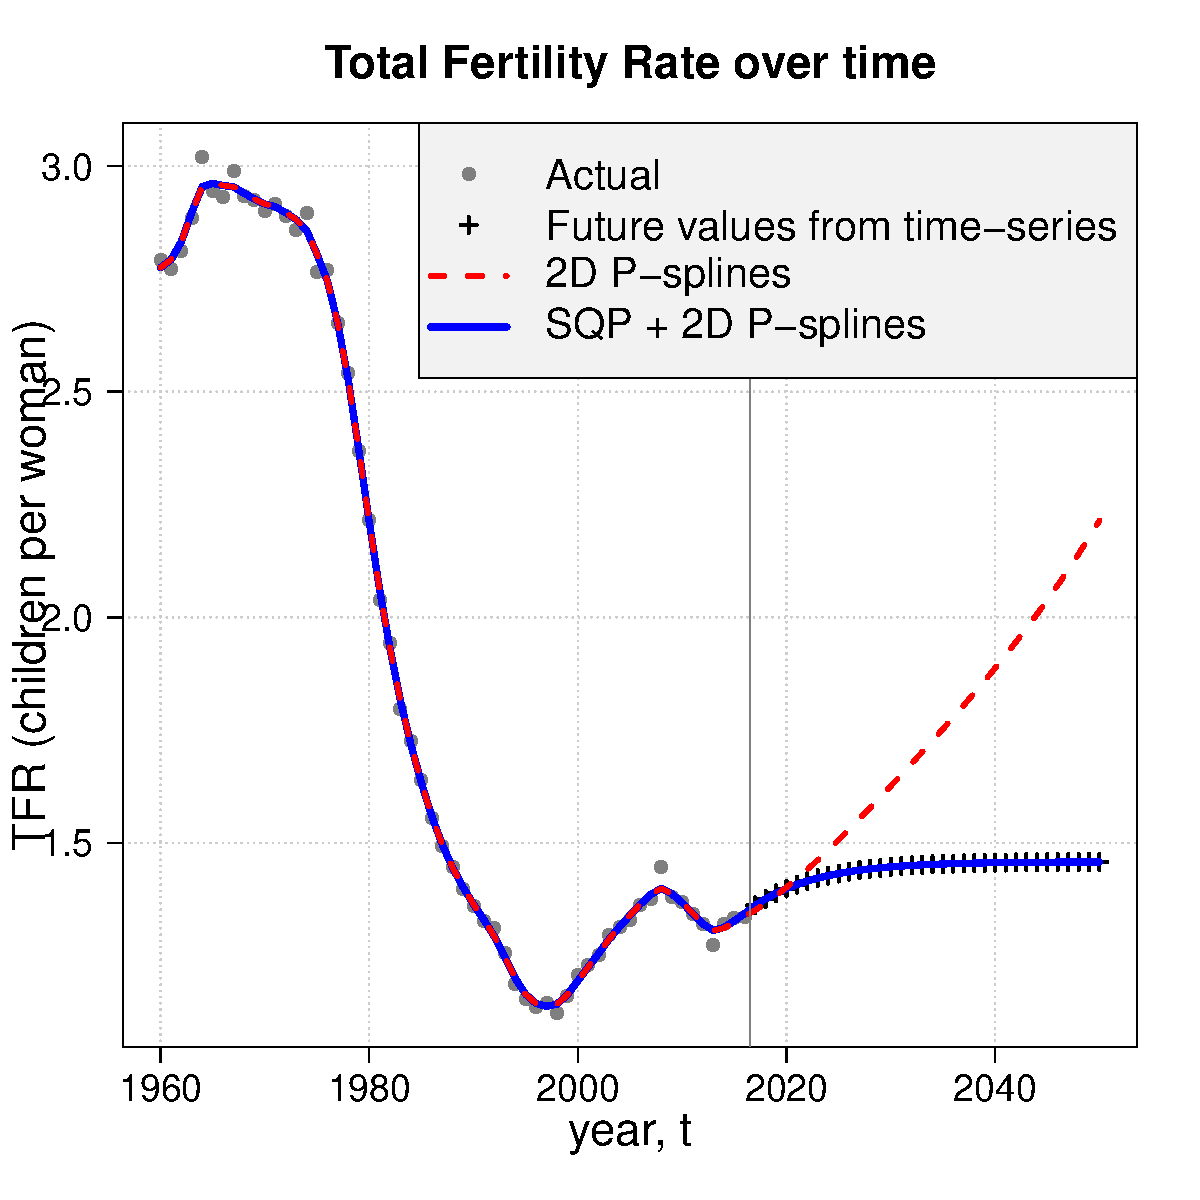
\includegraphics[scale=0.25]{CamardaTFR.pdf}
	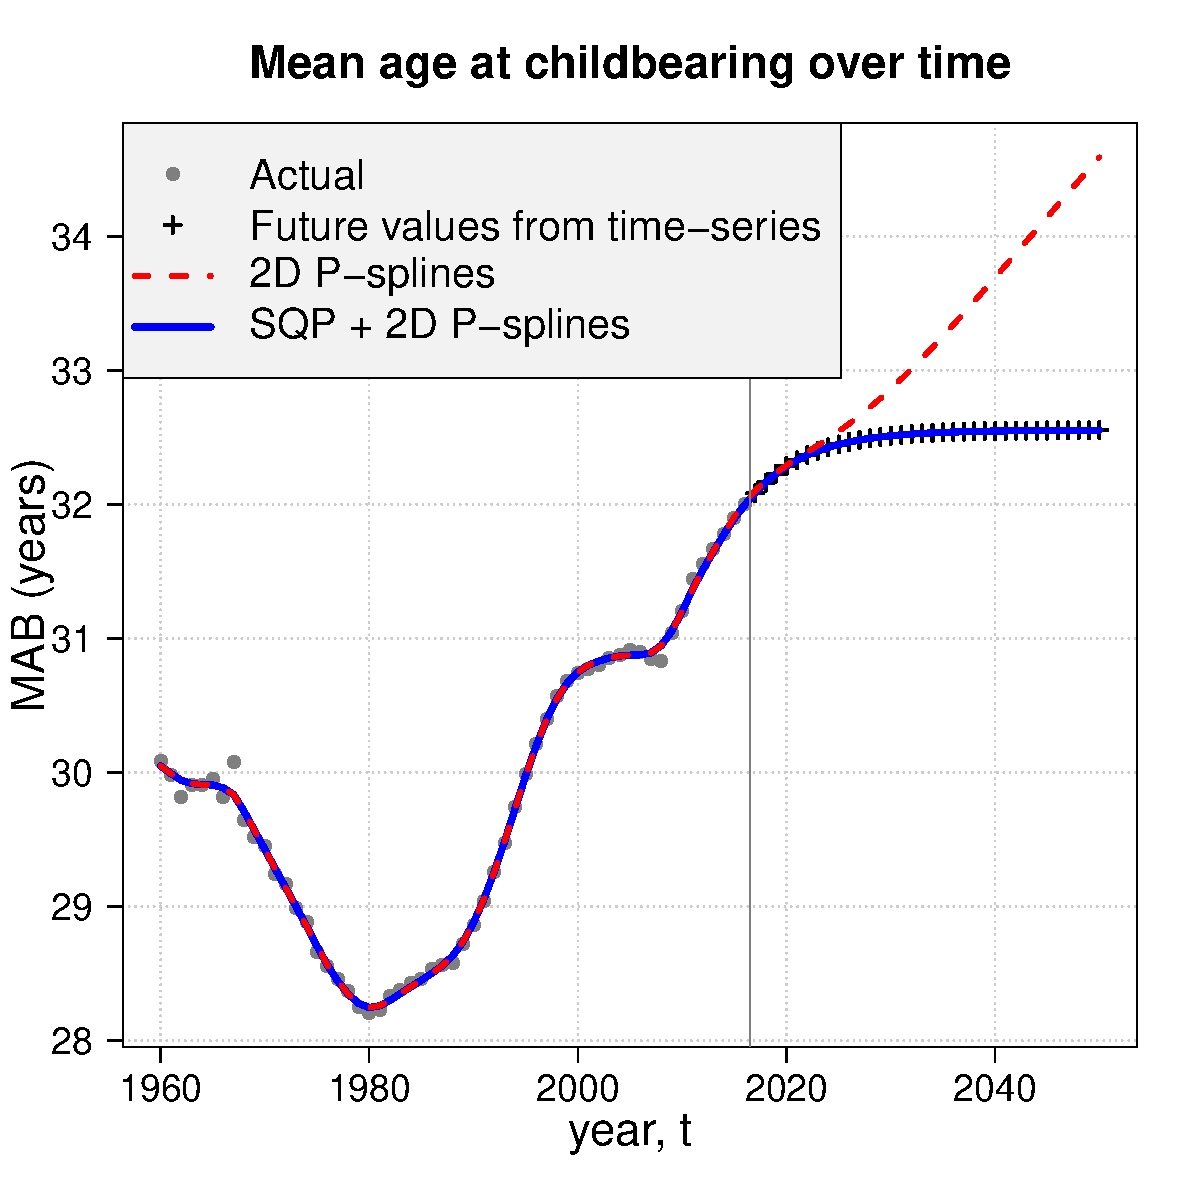
\includegraphics[scale=0.25]{CamardaMAB.pdf}
	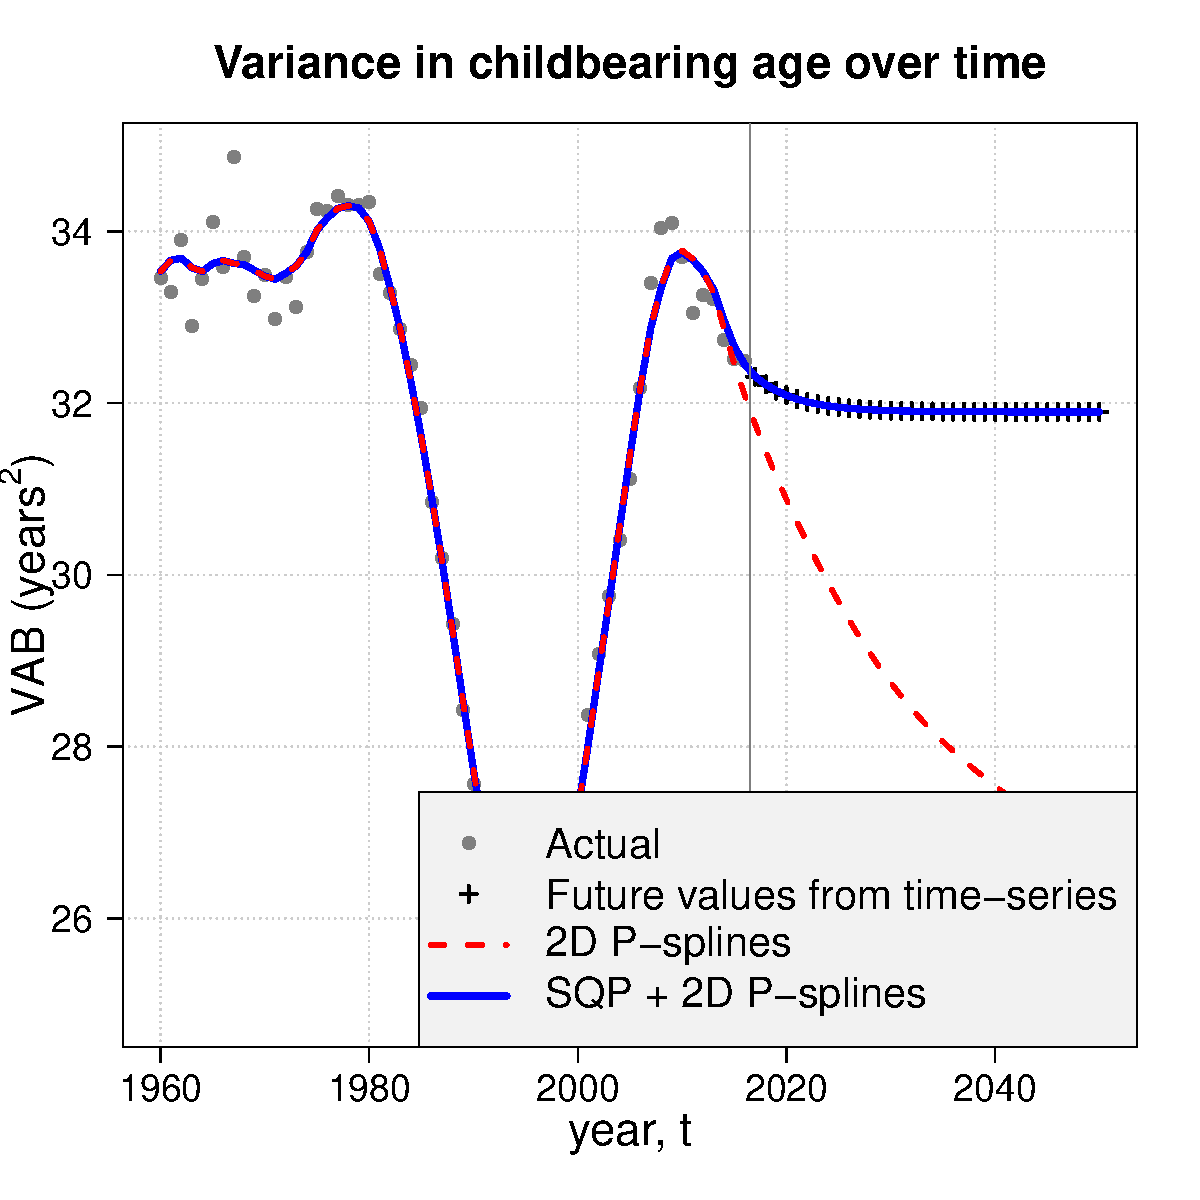
\includegraphics[scale=0.25]{CamardaVAB.pdf}
	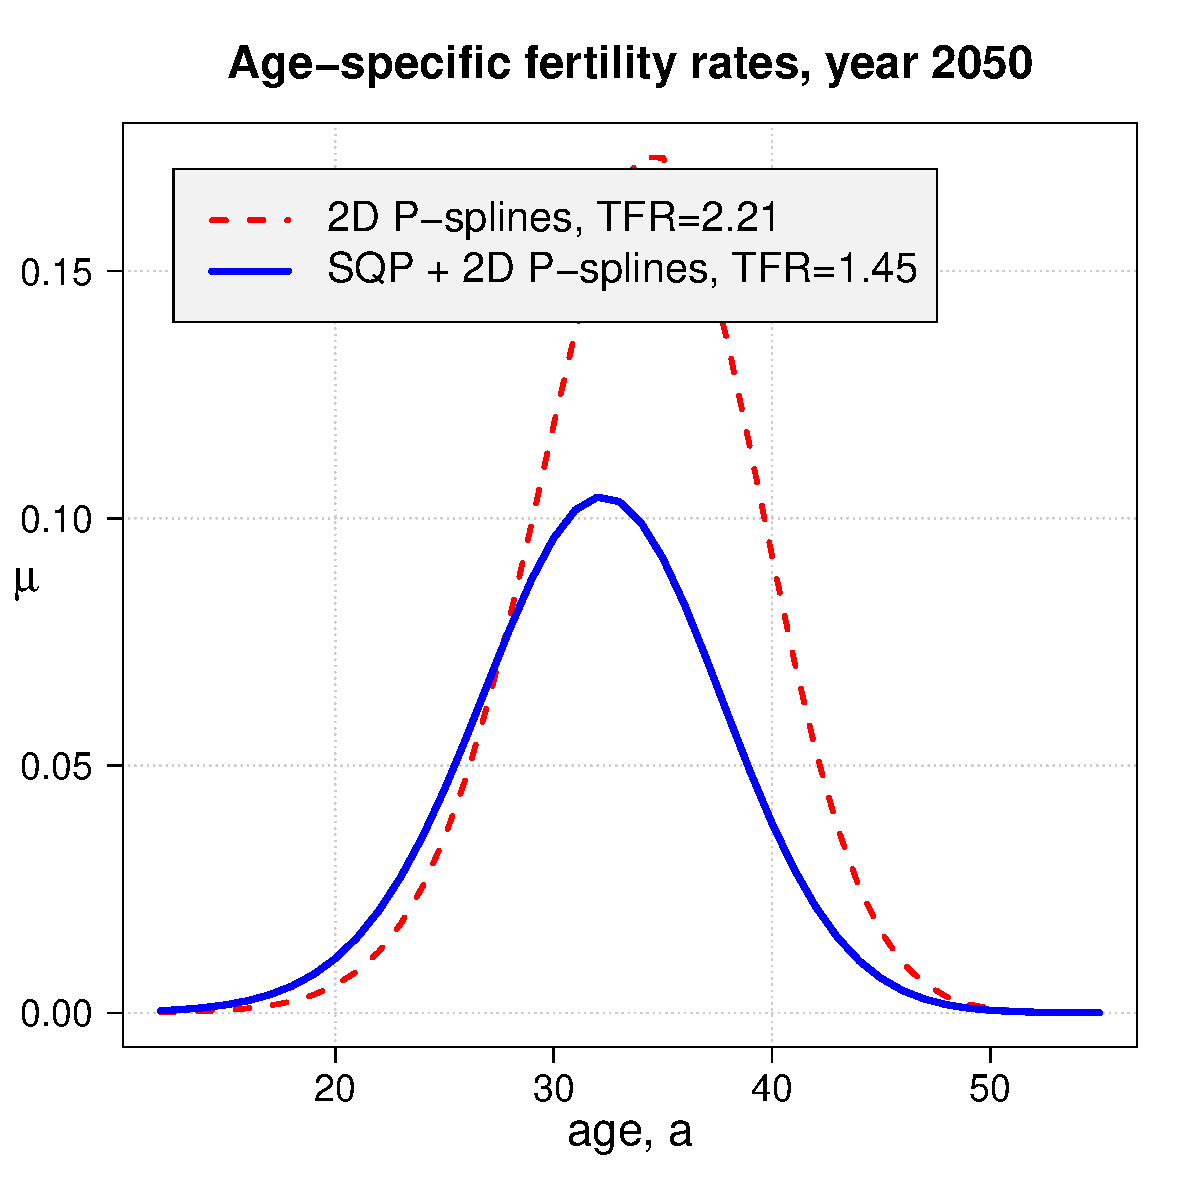
\includegraphics[scale=0.25]{CamardaFert2050.pdf}
	\caption{\label{fig:CamardaFert} Top and left-bottom panels: Actual, estimated and forecast Total Fertility Rate, Mean and Variance in childbearing age by time-series analysis, 2D $P$-splines and the SQP+2D $P$-splines. Right-bottom panel: Age-specific fertility rate in 2050 by 2D $P$-splines and the SQP+2D $P$-splines. Spain, ages 12-55, years 1960-2016, forecast up to 2050.}
\end{figure}

\references
\begin{description}
\item[Currie, I.~D. et al.]
	(2004). Smoothing and Forecasting Mortality Rates. {\it Statistical
	Modelling}, {\bf 4}, 279-298.
\item[Nocedal, J. \& Wright, S.~J.] (2006). {\it Numerical Optimization}. Springer.
\item[\v{S}ev\v{c}\'ikov\'a, H. et al.] (2016). 
Age-Specific Mortality and Fertility Rates for Probabilistic Population Projections. In R.~Schoen
(Ed.), {\it Dynamic demographic analysis}, 285\,--\,310. Springer.
\item[United Nations, Population Division] (2017). 
{\it World Population Prospects: The 2017 Revision, Volume II}. ST/ESA/SER.A/400.
\end{description}

%, Durb\'an, M. and Eilers, P.~H.~C.
% Li, N. Kantorova, V., Gerland, P. and Raftery, A.~E.

\end{document}

%Scenario-based projections could be also conveniently implemented using the proposed approach. 

%general model that allows to smooth and forecast future age-specific death and fertility rates complying summary measures such as life expectancy at birth and total fertility rates. 


%This study can be an elegant and convenient alternative to forecast vital rates without imposing strong structure on future mortality and fertility age-patterns. 

%Bayesian hierarchical models has been performed to obtain future life expectancy at birth and total fertility rates 
% for all countries in the world. Afterwards demographic models have been carried uut 
%mographers and actuaries have on future values of summary measures
%such as life expectancy at birth and total f

%On the one hand, vital rates are modelled using two-dimensional $P$-splines as in Currie et al.~(2004). On the other, summary measures are commonly nonlinear functions of the estimated penalized coefficients. Constrained nonlinear optimization is hence necessary and we extend a Sequential Quadratic Programming (SQP) procedure (Nocedal \& and Wright, 2006).  




%\begin{equation}\label{eq:SQLalg}
%\left[ \begin{array}{cc}
%\bm{L} & \bm{H}\\
%\bm{H}^{T} & \bm{0}_{n_{2} \times n_{2}}
%\end{array}\right]
%\left[ \begin{array}{l}
%\bm{\alpha}_{\nu+1}\\
%\bm{\omega}_{\nu+1}
%\end{array}\right] =
%\left[ \begin{array}{c}
%\bm{r} - \bm{L}\bm{\alpha}^{(\nu)}\\
%\bm{e}^{0}_{\mathrm{T}} - \bm{e}^{0} (\bm{\alpha}^{(\nu)})
%\end{array}\right] \, ,
%\end{equation}
%
%
%\begin{equation}\label{eq:SQLalg}
%\left[ \begin{array}{cl}
%\tilde{\bm{L}} & \tilde{\bm{H}}\\
%\tilde{\bm{H}}^{T} & \bm{0}_{n_{2} \times n_{2}}
%\end{array}\right]
%\left[ \begin{array}{l}
%\bm{\alpha}\\
%\bm{\omega}
%\end{array}\right] =
%\left[ \begin{array}{c}
%\tilde{\bm{r}} - \tilde{\bm{L}}\tilde{\bm{\alpha}}\\
%\bm{e}^{0}_{\mathrm{T}} - \bm{e}^{0} (\tilde{\bm{\alpha}})
%\end{array}\right] \, ,
%\end{equation}



The hat matrix is defined as
$$
H=X(X^\T X)^{-1}X^\T
$$
Please note we use \verb|^\T| to mean transposed matrices and vectors.

\subsection{Section 1.1}
Text for the first subsection within section 1. (Do you really need subsections ?)
\subsection{Section 1.2}
Text for the second subsection within section 1.
\section{Section 2}
Text for the second section. This section will have no subsections.



%***********************************************************************

% Tables can be included at any place in the text.
% As general format, use tables with horizontal lines only
% (i.e., no vertical lines separating columns).
% Start and end each table with a double horizontal line.
% Tables are incorporated using a table environment:

\begin{table}[!ht]\centering
	% A caption is put above the table and a label is defined
	% to be used for reference to this specific table.
	% Use labels which are very unlikely to be used by
	% other contributors; for example, use labels starting
	% with the surname of the first author.
	\caption{\label{smith:tab1} Caption text \textbf{ABOVE} the table.}
	% A table with three columns, where the first is left aligned,
	% the second has centred entries, and the third is right aligned,
	% is generated as follows (note: if requested, use \cmidrule{} instead of \cline{})
	\medskip
	\begin{tabular}{lcr}
		% First line:
		\toprule[0.09 em]
		% The body of the table:
		Title col1 & Title col2 & Title col3 \\
		\midrule
		row1 col1  & row1 col2  & row1 col3  \\
		row2 col1  & row2 col2  & row2 col3  \\ %
		row3 col1  & row3 col2  & row3 col3  \\
		% last line:
		\bottomrule[0.09 em]
	\end{tabular}
\end{table}

% In the text, reference to the Table can be made as follows:
We refer to Table~\ref{smith:tab1} for a summary of our main results. Have a look to Table~\ref{smith:tab2} for
an additional example.

\begin{table}[!ht]\centering
	\caption{\label{smith:tab2} Caption text \textbf{ABOVE} the table.}
	\medskip
	\begin{tabular}{lcr}
		% First line:
		\toprule[0.09 em]
		% The body of the table:
		&\multicolumn{2}{c}{Title  for cols 2 -3} \\
		\cmidrule{2-3} %
		Title1 & Title2 & Title3 \\
		\midrule
		& $a$  & $c$ \\
		& $b$  & $d$ \\ %
		\midrule[0 em]
		Total  & $a+b$  & $n$  \\
		% last line:
		\bottomrule[0.09 em]
	\end{tabular}
\end{table}



%***********************************************************************

% Figures can be included at any place in the text.
% The only allowed formats for figures are pdf files.
%
% Please, do not include figures in any other format.
%
% Use file names which are very unlikely to be used by
% other contributors; for example, use file names starting
% with the surname of the first author.
% Figures are incorporated using a figure environment:
% Make sure you specify the extension of the file (pdf)

Finally a figure (in \verb|.pdf|!)

\begin{figure}[!ht]\centering
	% You can pre-specify the width of the graph:
	\includegraphics[width=8cm]{castelo.pdf}
	% Below the figure, a caption is put, and a label is defined
	% to be used for reference to this specific figure.
	% Use labels which are very unlikely to be used by
	% other contributors; for example, use labels starting
	% with the surname of the first author.
	\caption{\label{smith:fig1} Caption text \textbf{BELOW} the figure.}
\end{figure}


% In the text, reference to the Figure can be made as follows:
We refer to Figure~\ref{smith:fig1} for a~graphical representation.


%***********************************************************************

%% Acknowledgments, if needed:
%\acknowledgments{Special Thanks to ... }

%***********************************************************************

% References should be placed in the text in author (year) form.
% The list of references should be placed below IN ALPHABETICAL ORDER.
% (Please follow the format of the examples very tightly).

%\item[Diggle, P.J., Liang, K-Y., and Zeger, S.L.] (1994).
%     {\it Analysis of Longitudinal Data}.
%     Oxford: Clarendon Press.
%\item[Green, P.J. and Silverman, B.W.] (1994).
%     {\it Nonparametric Regression and Generalized Linear Models}.
%     London: Chapman \& Hall.
%\item[Henderson, C.R.] (1973).
%     Sire evaluation and genetic trends.
%     In: {\it Proceedings of the Animal Breeding and Genetics Symposium in
%     Honour of Dr.\ L.\ Lush}, Champaign, Illinois, 10\,--\,41.
%\item[Lee, Y. and Nelder, J.A.] (1996).
%     Hierarchical generalized linear models.
%     {\it Journal of the Royal Statistical Society, Series B}, {\bf 58},
%      619\,--\,678.
%\item[Robinson, G.K.] (1991).
%     That BLUP is a good thing: the estimation of random effects (with Discussion).
%     {\it Statistical Science}, {\bf 6}, 15\,--\,51.
